\section{Data gathering}

From here, the procedure and the environment of gathering information to elaborate approaches will be discussed in detail.

\subsection{Test environment}

In order to find scan ranges that are likely to be answered positively, data from as many ECUs as possible is needed. In the context of the PetS3 project a remote testing environment has been created. This was particularly helpful in light of the contact limitations at the time of writing.

The infrastructure of Laboratory for Safe and Secure Systems (LaS3) was used for that. Specifically, their GitLab server was used, displayed in \autoref{fig:gitlab-screenshot}.

%GitLab screenshot
\begin{figure}[h]
    \centering
    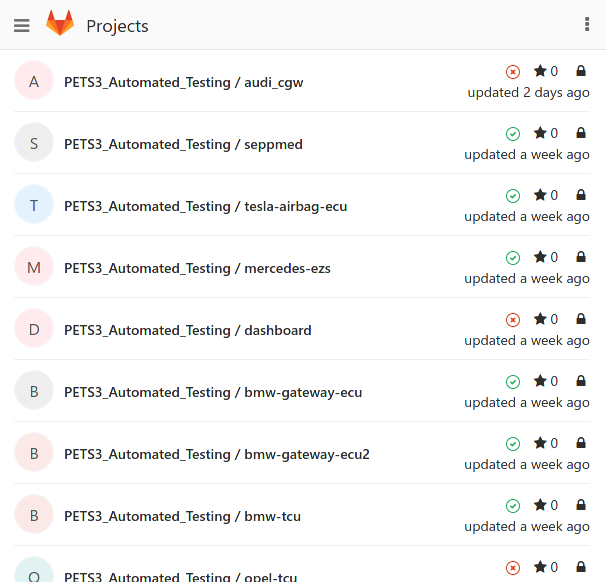
\includegraphics[width=0.7\textwidth]{gitlab-screenshot}
    \caption{Screenshot of the GitLab server.}
    \label{fig:gitlab-screenshot}
\end{figure}

Fourteen ECUs are available for testing on this server. Three of them are from Opel and thus only support GMLAN but not UDS.

For each ECU a YAML configuration file has been created. Various work is done here, for example installing this CAN-ISOTP module, if the running device is not at least on Linux 5.10 (see \autoref{sec:scapy}). Also, the current Scapy tree from the currently working branch is pulled and checked out.

Then, the actual tests are executed that are written in the pytest framework. Here, a UDS scan can be started. At the same time, another process is started to record all CAN traffic that takes place during the execution of the tests.

Finally, the resulting files are uploaded to the GitLab server so that they can be downloaded via a browser program.

\subsection{Explaining the stored data from one scan}

In total, five files are stored after a scan, which will be explained in this section.

\begin{itemize}
    \item candump.log
    \item generic.log
    \item profiling.csv
    \item milestones.csv
    \item data.pkl
\end{itemize}

The candump.log file is created by the candump program from the can-utils \cite{can-utils}. The generated files have a simple structure, each line representing one CAN packet.

\begin{samepage}
\begin{minted}{text}
(<timestamp>) <interface> <identifier>#<payload>
(1611779255.926425) can1 714#03225FB2CCCCCCCC
(1611779255.929936) can1 77E#037F2231AAAAAAAA
(1611779255.935338) can1 714#03225FB3CCCCCCCC
(1611779255.940680) can1 77E#037F2231AAAAAAAA
\end{minted}
\end{samepage}

Unfortunately, these resulting files contain a lot of information that is not only not needed, but also unwanted, as it leads to more difficult analysis and to higher storage usage. \autoref{fig:can-unwanted-information} shows the unnecessary information as it is ECU specific and does not add any value for the analysis.

%CAN unwanted information
\begin{figure}[h]
    \centering
    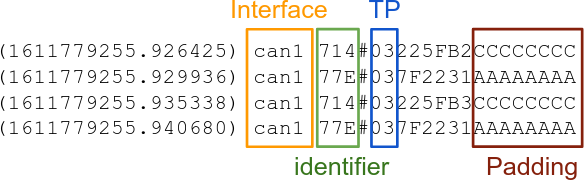
\includegraphics[width=0.7\textwidth]{can-unwanted-information}
    \caption{ECU specific information. TP = Transport protocol information}
    \label{fig:can-unwanted-information}
\end{figure}

Consequently, an abstraction is desirable. The newly created format is called the generic format. It removes the interface, the padding, resolves the transport protocol information (ISOTP) and replaced the identifier with mnemonics (s = Server, c = Client). Each line represents a full UDS packet, instead of a CAN packet as in the candump logs. \autoref{fig:candump-generic-conversion} illustrates the input and output of a conversion.

%candump to generic conversion
\begin{figure}[h]
    \centering
    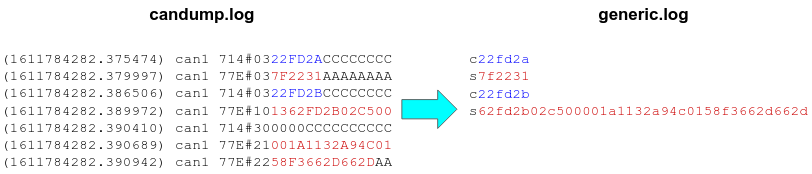
\includegraphics[width=1\textwidth]{candump-generic-conversion}
    \caption{candump.log to generic.log conversion.}
    \label{fig:candump-generic-conversion}
\end{figure}

This format proved to be very useful as it allows quick analysis by chaining common Linux programs.

For instance, counting the number of requests of one scan is a single command:
\begin{samepage}
    \begin{minted}{bash}
        $ grep '^c.*' -c generic.log
        988844
    \end{minted}
\end{samepage}

For profiling, two csv files have been added as output for the UDS scanner, namely profiling.csv and milestones.csv.

The former contains which enumerator ran under which state and when. It contains a fairly simple format, only containing the expected information:

\begin{samepage}
    \begin{minted}{text}
        state     ,enumerator       ,start            ,end
        ECU Reset ,ECU Reset        ,1611770228.135198,1611770228.658480
        [session1],UDS_CCEnumerator ,1611770228.661016,1611770231.236505
        ECU Reset ,ECU Reset        ,1611770231.236789,1611770231.754865
        [session1],UDS_DSCEnumerator,1611770231.756320,1611770231.895722
    \end{minted}
\end{samepage}

Each line in the milestones.csv contains a timestamp and the name of the final state of a found state path and its timestamp:

\begin{samepage}
    \begin{minted}{text}
        session1   ,1613302518.995168
        session2tp1,1613302569.605534
        session1tp1,1613309304.481464
        session3tp1,1613310988.231891
    \end{minted}
\end{samepage}

From this follows that a name can occur multiple times in this file, if there are more paths to the same state. What path will be taken is decided later in the UDS scanner after detecting it with the Dijkstra algorithm to find the shortest path.

Last but not least, the data.pkl file. Pickle is the object serialization module of the Python Standard library \cite{pickle}. The data.pkl file is the UDS scanner object after the scan, thus containing all results. This is helpful for debugging, analysis and also for simulation.

\subsection{Profiling the UDS Scanner}

The Pareto principle indicates that small number of causes can be responsible for a large percentage of effects \cite{pareto}. This is also applicable to optimization problems. Usually only a few number of code lines are responsible for the majority of the runtime. Optimizing them is far more effective than performing micro-optimizations as they naturally improve the performance to a great extent. Moreover, micro-optimizations are usually even more difficult to accomplish.

This is where the profiling.csv and the milestones.csv come into play to profile the UDS Scanner to find those places in need of optimization.

These files are used to create Gantt charts that show which parts of the UDS scanner take up most of its runtime. All diagrams in this work, including the Gantt charts, are generated with the library plotly for Python \cite{plotly}.

These Gantt charts have been created for each available ECU. For illustration one is sufficient since each chart showed the same gist (see \autoref{fig:tesla-gantt}).

\begin{figure}[h]
    \centering
    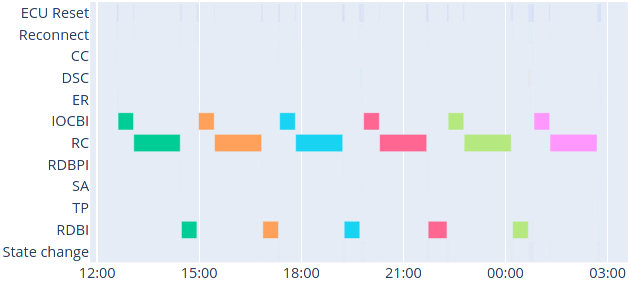
\includegraphics[width=1\textwidth]{tesla-gantt}
    \caption{Gantt chart of the Tesla-Airbag-ECU.}
    \label{fig:tesla-gantt}
\end{figure}

The time is represented on the x-axis and the enumerators and events are listed on the y-axis. One color represents one state of the ECU.
Although it seems that some enumerators and events do not require time, their time consumption is only so small that they are not or hardly visible in this scaled-down version of the diagram.

The main cause of runtime is the UDS\_RCEnumerator. This was expected, since this is the enumerator with the most generated requests. In second place are the UDS\_IOCBIEnumerator and the UDS\_WDBISelectiveEnumerator. The latter consists of actually two enumerators, the UDS\_RDBIEnumerator and the UDS\_WDBIEnumerator. The UDS\_RDBIEnumerator generates more requests than the UDS\_WDBIEnumerator to a large extent, which accordingly hardly contributes to the runtime. Therefore, for simplicity, this enumerator will be called UDS\_RDBIEnumerator from here on.
The UDS\_IOCBIEnumerator and UDS\_RDBIEnumerator generate about the same runtime, this was to be expected since they generate the same number of requests. The RDBI service is much more frequently supported by ECUs than the IOCBI service, resulting in a smaller database, so it was decided that the RDBI service would be optimized instead of the IOCBI service.

In summary, the UDS\_RCEnumerator and the UDS\_RDBIEnumerator are the most critical performance barriers of the UDS scanner and therefore belong to the subjects to optimize.
